\documentclass[letterpaper,12pt]{article}
\usepackage{apacite,pdfpages,enumitem,fancyhdr,url,graphicx,tabularx,ragged2e,booktabs,caption,epstopdf}
%http://www.ctan.org/tex-archive/biblio/bibtex/contrib/apacite/apacite.pdf
\usepackage[top=1in, bottom=1in, left=1in, right=1in]{geometry}
\usepackage[doublespacing]{setspace}
\pagestyle{fancy}
\setlist{nolistsep}
\setcounter{secnumdepth}{0}
\setlength{\skip\footins}{1.2cm}
\raggedbottom
\widowpenalty=1000
\clubpenalty=1000
\lhead{Bias in Published Academic Papers from Gaps in a Public Reddit Archive}
\rhead{\thepage}
\cfoot{}
\title{Bias in Published Academic Papers from Gaps in a Public Reddit Archive}
\date{17 November 2016}
\author{Devin Gaffney and Nate Matias}
\begin{document}
\maketitle
\doublespacing
\section{Abstract}
On July 2, 2015, Jason Baumgartner, known as /u/Stuck\_in\_the\_Matrix on Reddit, published a dataset claimed to comprise ``every publicly available Reddit comment'', which was quickly shared on Bittorrent and the Internet Archive. Within a short period, the data became the basis of a series of academic papers on topics including machine learning, social behavior, politics, breaking news, and hate speech. When exploring this data in our own research, we discovered substantial gaps and limitations in the dataset which may contribute to bias in the findings of research that relies on it. This report documents our work to identify those gaps and consider the risks to research validity that they represent. In summary, we identify strong validity risks to research that considers user histories or network analysis, moderate risks to research that relies on sums of participation, and minimal risk to machine learning research that trains models from content analysis rather than making representative claims about behavior and participation on Reddit.

\section{The Baumgartner Dataset}

Trace data sourced from online platforms has become an essential component for many forms of research ranging from sentiment analysis \cite{pak2010twitter} to epidemiological modeling \cite{abdullah2011epidemic} and economics \cite{bollen2011twitter}. Dominant social platforms such as Twitter and Facebook have provided researchers with opportunities to directly study complex phenomena that, at their root, rely strongly on the nature of social interaction \cite{bond201261}. The reason for this, as \citeA{tufekci2014big} argues, is that large platforms (specifically Twitter, in this analogy) serve as a \textit{model organism} for the social sciences, one that allows for ideal conditions for measurement of many phenomena in a relatively accessible form. On July 2, 2015, a new model organism was provided to researchers by Jason Baumgartner -- a ``complete'' copy of one of the largest forums, Reddit, which has gained high visibility in the past several years due to events such as the Reddit blackout \cite{matias2016going,newell2016user,baumgartner2015dataset} and the Gamergate controversy \cite{massanari2015gamergate}. Subsequently, many researchers have adopted the dataset, and have used it's unique affordances to study the evolution of social networks \cite{fire2016time,fire2016analyzing} and user migration through online platforms \cite{tan2015all,newell2016user}. Aside from the technical differences in terms of the architecture of this platform as compared to other platforms dominant in research, the distinguishing factor of the Baumgartner Reddit dataset is it's completeness, which allows for a higher degree of validity in findings which need not have any ambiguities about how unsampled data may differ from samplings typically present in research on other platforms \cite{lotan2011arab}. This dataset, however, is not actually complete.

\subsection{Sequential ID Analysis}

The reason that the entire contents of the platform could be systematically collected, and the reason that it has been shown that the dataset is in fact not complete. Many databases include the concept of an Identity column, or a column that generates an internal ID to serve as a unique reference to the row, or object, within the database. In many cases, this value auto-increments -- the first value in the database assumes a value of 1, the next, a value of 2, and so forth. This number can be artificially shifted within the space -- for instance engineers may partition early IDs of 1-1,000,000 for experimenting with data, for some reason, and start all real data created by users with ID 1,000,001. Barring this, however, if an object contains an ID of \textit{n}, then it is plausible to assume that there are at least \textit{n} objects within the database. By personal correspondence, Baumgartner has explained that this intuition led to the development of the systematic collection of all data on Reddit -- the algorithm batches up 100 integers, converts them to the Base 36 representation that Reddit uses to represent their objects, and then queries for those objects -- found objects will be returned by the request. This can be run in a highly parallel environment -- many batches of 100 IDs can be concurrently requested, with no need to interact with one another. On many platforms, some error may be returned if the data has been deleted -- with Reddit, no error is returned -- instead, a truncated object reflecting this deletion has occurred is returned. Therefore, barring technical issues, there should be a complete accounting for every ID within the range 1-\textit{n} for all comments and submissions within the dataset, which allows for a validity check of the completeness claim.

\section{Diagnosing Missing Data}

The completeness problem was found relatively early in working with the data -- a random sample of subreddits was selected, and a timeline was generated for the daily counts of comments and submissions on the subreddits. Plots showed impossible results given the architecture of Reddit -- some comment timelines started earlier than their corresponding submission timelines. On Reddit, comments can only refer to other comments or submissions, therefore, a submission would have to exist in order for a comment to subsequently refer to it, and the order of these events is unidirectional with respect to time. Digging further, many instances of references to missing data begun to appear throughout the data. An exhaustive search through the data was therefore necessary. 

Two sets of data within the dataset, comments, and submissions, ultimately have been shown to be missing data. Current work on this front has uncovered two issues with the data currently referred to as the ``known unknowns'' and the ``unknown unknowns''. Known unknowns are comments which refer to other comments or parent submissions, but the referred-to comment or parent submission is not contained within the Baumgartner dataset. ``Unknown unknowns'' are cases where there are gaps within the ID space of the Baumgartner dataset. The earliest comment in the  Baumgartner dataset is comment \#2, which allows for us to know that, between the oldest and the newest within the dataset, there are 943,755 total ``gaps'', or number of missing comments (which could be a known unknown, a truly unknown unknown comment that can be mined, or content not available for technical reasons (deleted data on Reddit is validly returned by the Reddit API, and included in the data as a deleted record)). Submissions are much trickier. While there are 943,755 ``gaps'' in the space of IDs for submissions, the first submission in the Baumgartner dataset starts at \#9,970,002 -- many small checks between \#1 and \#9,970,001 have been conducted, and submissions found, which suggests potentially significant problems with the collection process particularly in the early development of the forum. 
\begin{table}
  \begin{center}
    \begin{tabular}{ |c|c|c| } 
      \hline
      Data Type & Known Unknowns & Unknown Unknowns \\
      \hline
      Comments & 101,257 & 943,755 \\ 
      Submissions & 405,911 & 1,539,583 \\ 
      \hline
    \end{tabular}
  \end{center}
  \caption{Totals for missing data in the Baumgartner dataset}
  \label{table:total_missing}
\end{table}

\begin{figure}[h]
  \centering
  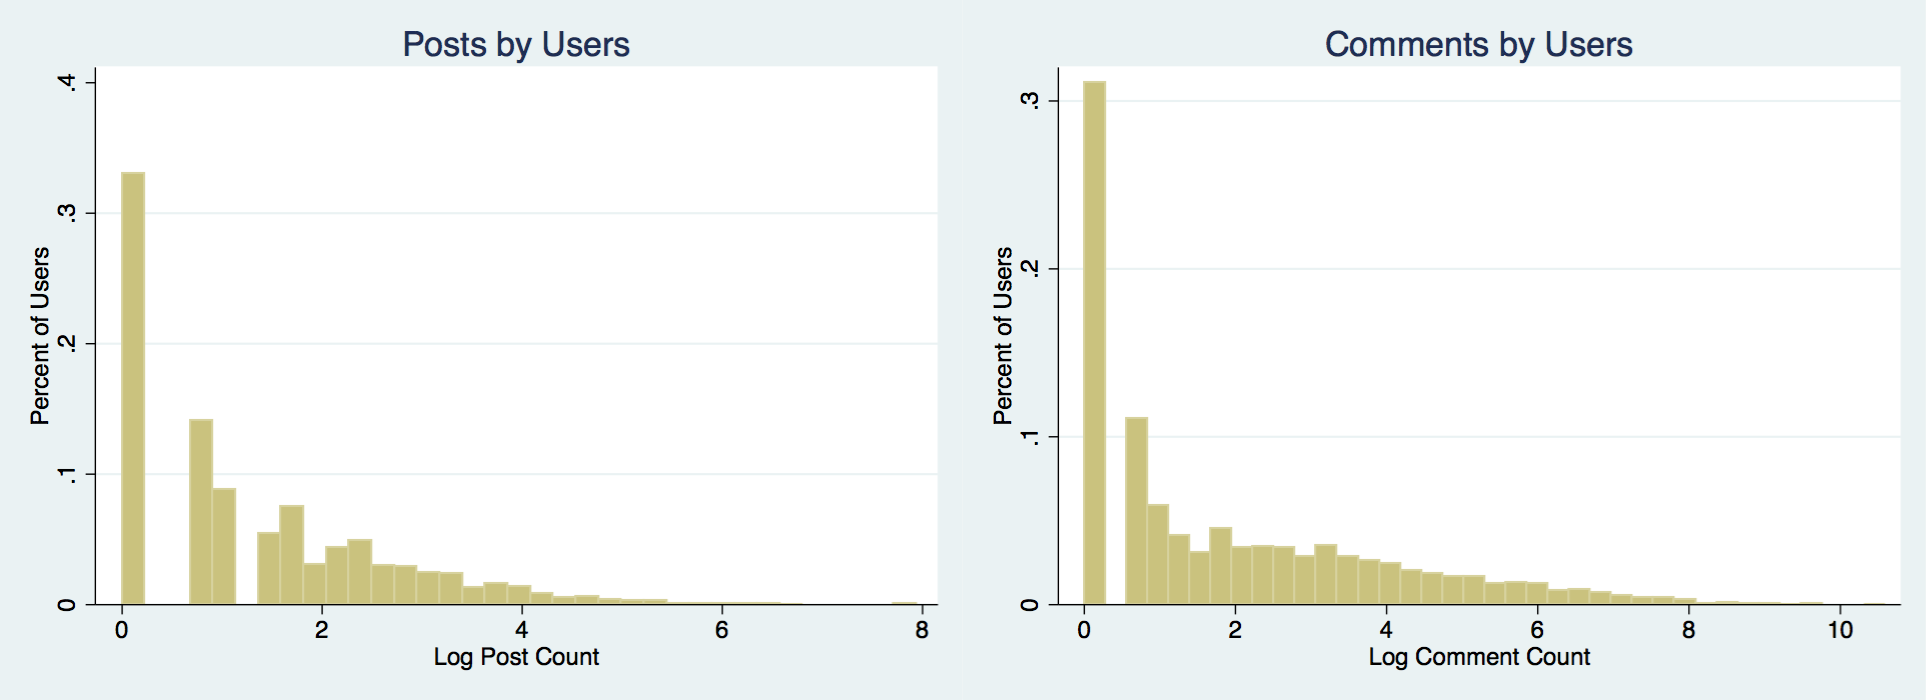
\includegraphics[width=\textwidth]{post_counts}
  \caption{Histograms of sampled user Submission and Comment counts}
  \label{fig:post_counts}
\end{figure}

\subsection{Rough Estimates}

A random sample of 7,400 accounts were selected from the Baumgartner dataset, and summary statistics were generated for the users -- the average user posts 6.8 times and comments 96.6 times, though this is a highly skewed distribution, as the log-histograms in \ref{fig:post_counts}. Based on table \ref{table:total_missing}, the known maximum amount of missing comments and submissions is 943,755 and 1,539,583, respectively -- ``known unknowns'' are a subset of ``unknown unknowns''. Across the platform, this is, admittedly, a very small amount of missing data -- Across the entire Baumgartner dataset, only 0.043$\%$ and 0.65$\%$ of comments and submissions, respectively, are missing. The issue has a compounding effect, however: the skewedness of the dataset shows that a small number of users create a large amount of the content on the platform -- the more posts and comments they generate, ceteris paribus, the more likely their histories will be affected by the missing data issue.

Conservatively, we can provide a rough accounting for the qualitative degree to which this could affect a wide range of research by considering rough probabilities of data loss for individual Redditor histories. In reality, the missing data is far from uniformally distributed through the corpus, but relaxing this fact, we can simply compound probabilities to assess the degree to which a user could be affected by only a small amount of missing data. Using the averages from earlier, we can calculate the risk of any individual submission $r_s$ or comment $r_c$ being missing  simply by $\sum_c^n r_c$ and $\sum_s^n r_s$, respectively. In this case, the ``average'' Redditor may be exposed to a total maximum risk level of $\propto$ 4.18$\%$ likelihood for missing at least one comment and $\propto$ 4.46$\%$ for missing at least one submission. In the 7,400 individual set, approximately 2$\%$ of the sampled users had a 50$\%$ or greater chance of having a missing comment, and 2.6$\%$ of the sampled users had a 50$\%$ or greater chance of having a missing submission. These are only very rough approximations to help get a qualitative sense of how this missing data issue may create an appreciable problem for some forms of research -- a more considered typology of errors is considered below.

\subsection{Error Distribution}

Far from being uniformally distributed throughout the dataset, the instances of missing data are very bursty. This creates spaces within the data where the issue of missing data may be less of an issue or considerably more of an issue. Importantly, significant gaps were found for comments created around the time of the SOPA/PIPA protests \cite{benkler2015social}, while significant gaps in submissions were found in the months leading up to the Reddit blackout \cite{matias2016going}, though this work falls short of drawing any direct causal inference in these two cases.

\begin{figure}[h]
  \centering
  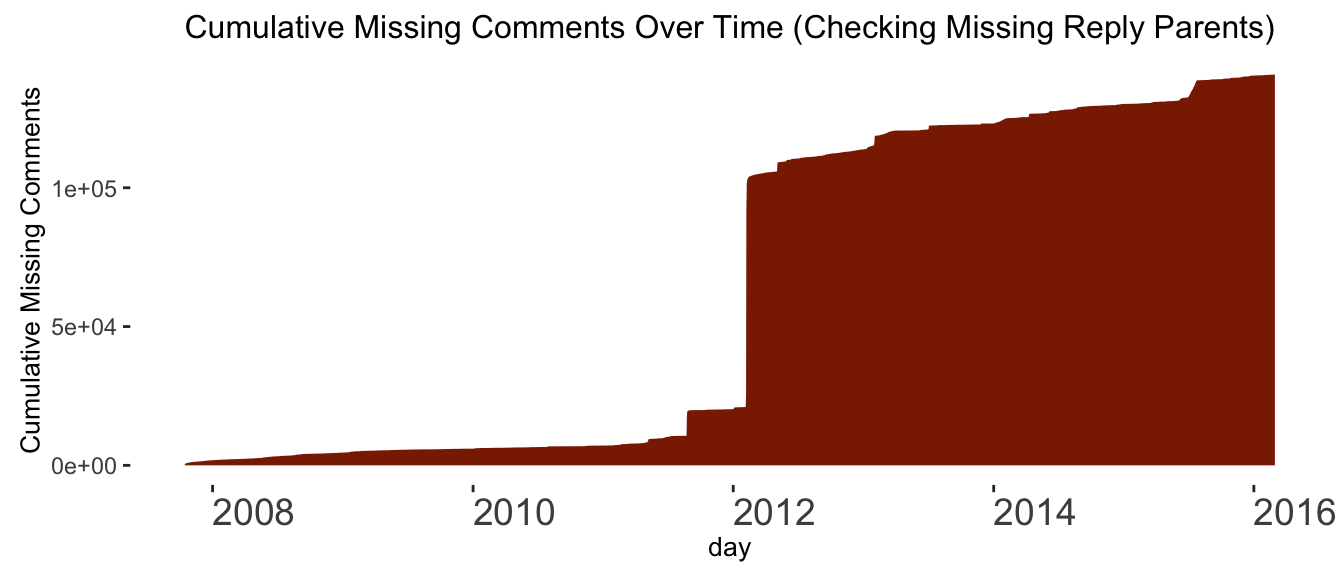
\includegraphics[width=\textwidth]{cumulative_missing_comments_time}
  \caption{Cumulative missing comments by dates of ``known unknowns'' referencing missing comments. Note the steep rise in 2012.}
  \label{fig:cumulative_missing_comments_time}
\end{figure}

\begin{figure}[h]
  \centering
  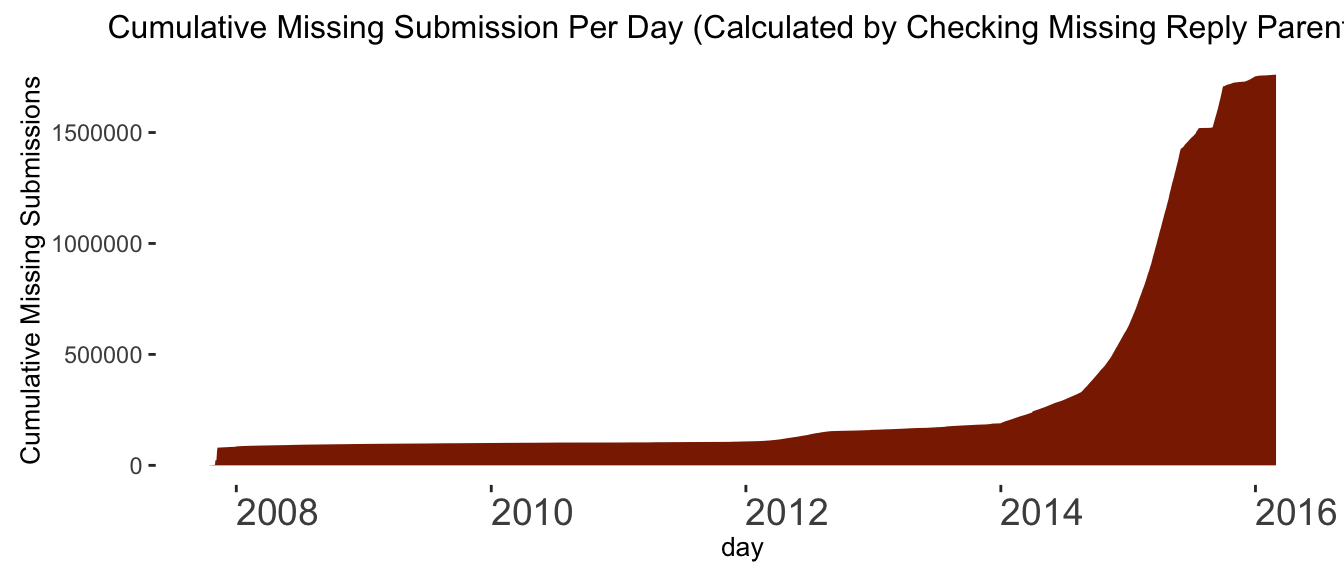
\includegraphics[width=\textwidth]{cumulative_missing_submissions_time}
  \caption{Cumulative missing submissions by dates of ``known unknowns'' referencing missing submissions. Note the steep rise over months leading to February 2016.}
  \label{fig:cumulative_missing_submissions_time}
\end{figure}

\begin{figure}[h]
  \centering
  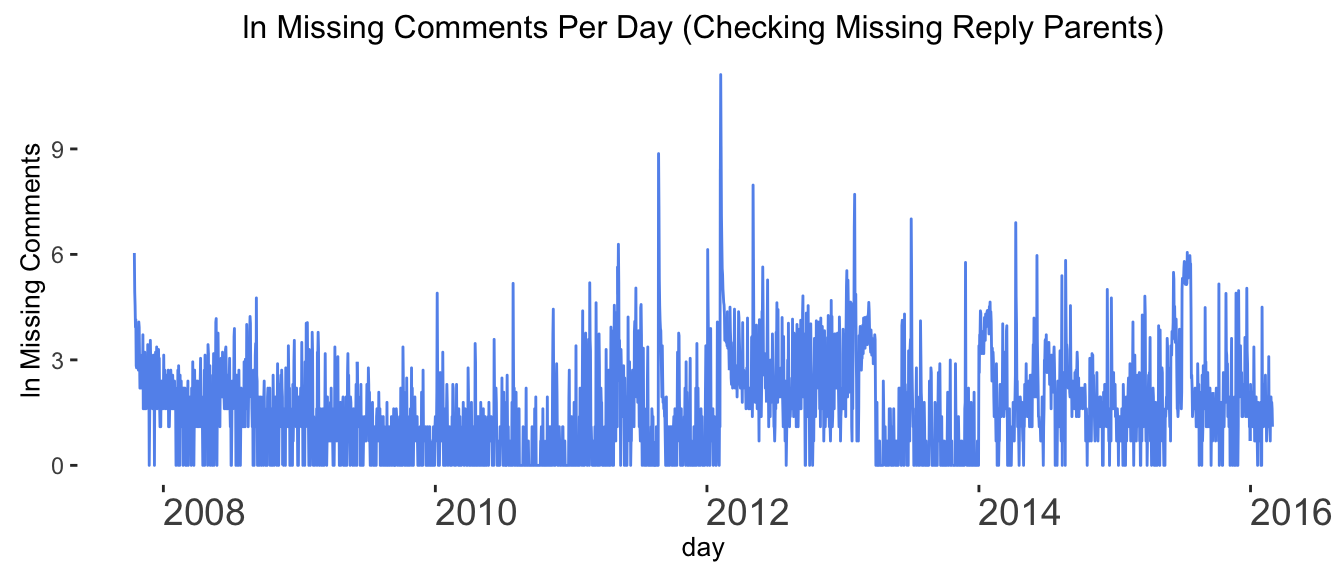
\includegraphics[width=\textwidth]{log_missing_comments_time}
  \caption{Log plot of missing comments over time - notice extremely large gaps by peaks that reach several orders of magnitude larger for brief moments.}
  \label{fig:log_missing_comments_time}
\end{figure}

\begin{figure}[h]
  \centering
  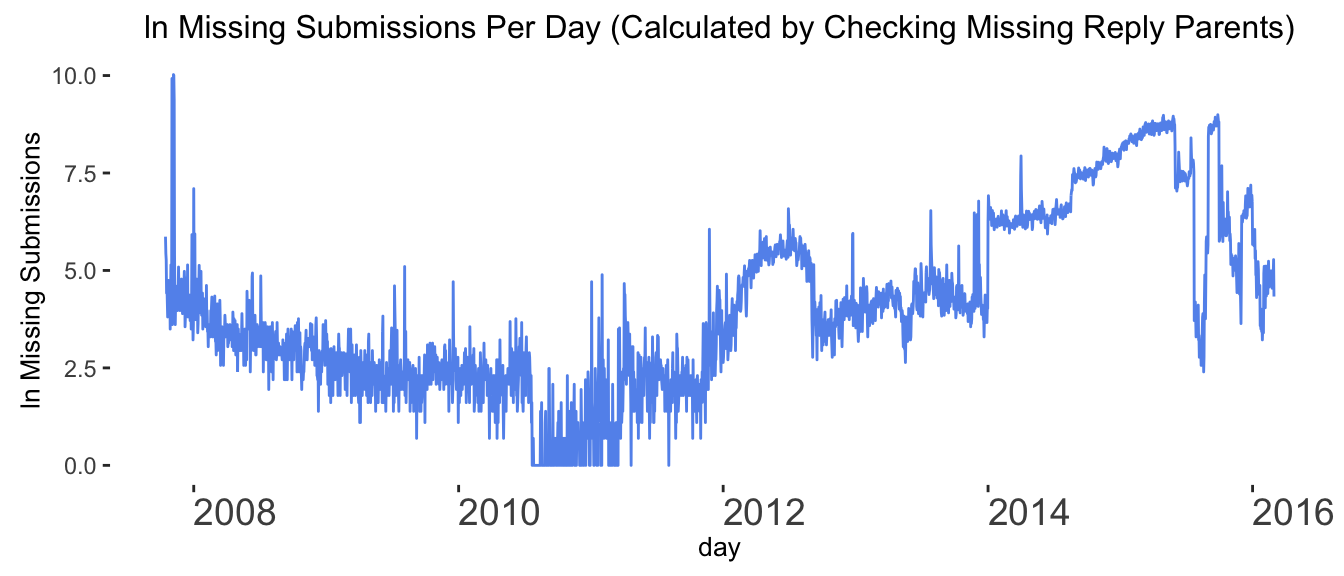
\includegraphics[width=\textwidth]{log_missing_submissions_time}
  \caption{Log plot of missing submissions over time - notice extremely large gaps by peaks that reach several orders of magnitude larger for brief moments.}
  \label{fig:log_missing_submissions_time}
\end{figure}

Overall, figures \ref{fig:log_missing_submissions_time}, \ref{fig:cumulative_missing_comments_time}, \ref{fig:cumulative_missing_submissions_time}, and \ref{fig:log_missing_comments_time} illustrate an erratic distribution of errors throughout the dataset -- and they appear to occur directly within time spaces of inherent research interest, which may affect results found by several works already \cite{matias2016going,newell2016user}. As alluded to earlier, some methodological designs may be affected more significantly by these issues than others that range from strong risks to minimal risks. Reviewing current literature that has used this dataset, it is possible to convey these issues as a typology of methodological concerns.

\section{Typology of Errors}

\textbf{User history analysis} papers also face the \textbf{highest risks}, since a missing comment or submission could hide an important part of that user’s history. A network analysis may fail to include a user’s participation in a particular community or interaction with a key user. Furthermore, survival analyses might mis-estimate the moment of departure or participation levels due to gaps in the dataset. \textbf{Network analysis} papers face \textbf{high risks}, since the presence or absence of a tie could be dependent on the missing data. \textbf{Sum analyses} that count the size or incidence rate of participation in subreddits or the use of certain kinds of language face \textbf{moderate risk}, especially when analyzing small communities and rare events. \textbf{Content analysis} that involves training machine learning systems on Reddit comments face \textbf{minimal risk} because their systems rarely make claims about the population of Reddit users.

\subsection{User History Analysis}

Papers that test hypotheses based on user histories that may have substantial gaps in them. Analyses that are especially sensitive to high-volume users are more likely, on average, to consider users whose histories have gaps. \citeA{hessel2016science}, for example, observes and compares sums of comment participation between subreddits, and observes the full chain of user history -- \citeA{hessel2015democrats} continues with a similar approach. \citeA{barbosa2016averaging} compares year cohorts of individual-level behavior across all of Reddit, and as has been shown, some years are more affected than others. Additionally, the large amount of potential missing submissions from Reddit's inception may also affect these findings. Depending on how the missing data is missing beyond what has already been shown, some findings may be substantially affected when using this methodology.

\subsection{Network Analysis}

Some papers test network hypotheses by constructing interaction networks between users or communities, sometimes over time. Gaps represent a high risk to these papers, since missing submissions may result in unobserved ties in the network. \citeA{tan2015all} observes histories of user accounts participating in different communities, while \citeA{fire2016analyzing} and \citeA{fire2016time} observe network ties over time modeled on user histories. Again, significant blocks of missing data, along with the potentially large amount of missing submissions from Reddit's nascency present potential issues to validity.

\begin{figure}[h]
  \centering
  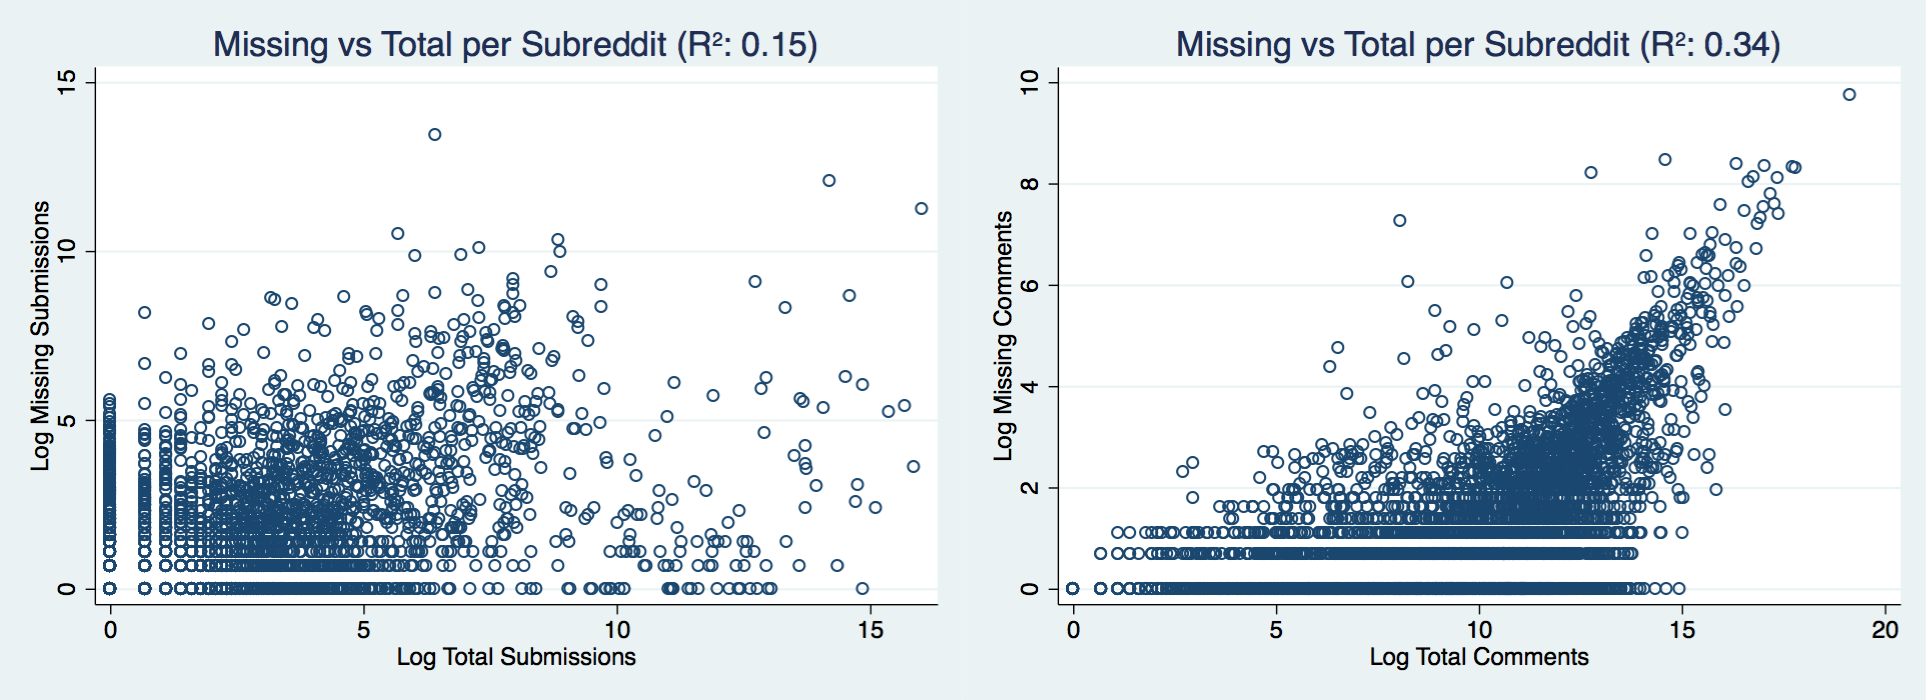
\includegraphics[width=\textwidth]{missing_count_total_count_correlation}
  \caption{Correlations between the size of subreddits according to total historical counts of comments and submissions versus observed known unknowns by subreddit - comments are mildly correlated, while submissions are not very correlated.}
  \label{fig:missing_count_total_count_correlation}
\end{figure}

\subsection{Sums of Participation}

Other papers test hypotheses based on participation sums within communities. Gaps that are biased toward particular communities will represent a risk to the validity of these studies. \citeA{matias2016going} observes levels of subreddit participation by moderators, observes relative participation levels of subreddit commenters in other subreddits, and observes moderator participation in ``metareddits''. \citeA{newell2016user} observes comment volumes within subreddits. \citeA{pew2016reddit} observes comments about political candidates across Reddit during a period where many submissions are within the dataset. \citeA{barbaresi2015collection} analyzes German language text to identify relative commenting rates about places in Germany. While in this instance, where /r/de shows only small amounts of known unknown comments (12) and submissions (450). 

Figure \ref{fig:missing_count_total_count_correlation} shows a deeper introspection -- a null hypothesis would state that the number of missing comments and submissions would be tightly correlated to the size of the subreddit. While a simple statistical regression between the total counts of missing data and known data shows the relationship to be significant, the $R^2$ is low enough in both cases to certainly conclude that studies on some subreddits could lead towards very biased results due to higher than random amounts of missing data - in practice, there are 78 subreddits where at least 20$\%$ of the comments are missing, and 1,755 subreddits where at least 20$\%$ of the submissions are missing -- of subreddits that have any missing data according to known unknowns, on average they are missing at least 35$\%$ of their submissions.

\subsection{Content Analysis}

Finally, some studies train machine learning models and conduct linguistic analysis of the Baumgartner dataset. Insofar as these studies do not make claims about populations, gaps represent a minimal risk to the validity of this research. \citeA{saleem2016web} trains machine learning models on comments from particular subreddits. Though the missing data is non-uniformally distributed over time, and mildly non-uniformally distributed across subreddits, it is unlikely that it favors any form of content over another. \citeA{saleem2016web}'s work is specifically focused on communities that have since been quarantined or banned, however, and from a qualitative review of where the mass of missing data is pooled, it seems to trend towards such communities -- across the three subreddits considered in their work, one of those subreddits actually has 696,642 comments that reference missing submissions, and only 606 known submissions (on that particular subreddit, however, only 1,100 of 1,585,014 comments were known to be missing). Again, as stated in the previous section, particular subreddits may have larger issues than others. Still, with a large enough corpus of training, it is likely that there is no bias about \textit{which} specific pieces of content are missing within most selection frames, so there is a minimal risk for work employing content analysis given a sufficient scale.

\section{Going Forward}

These issues have all been raised in direct with Baumgartner, whom has graciously and quickly made large strides in addressing these issues, and re-processing missing data. By publication time of this paper, it is likely that the issue will have been fully addressed, and the data re-published. In terms of what steps must be taken forward in increasing the integrity of this dataset, little is left and all steps forward are known. The other larger discussion, however, is about the role researchers play in vetting datasets sourced from non-academic providers. All datasets, just by nature of operationalizing a concept for the purpose of research, will have biases present -- in the process of designing research, these biases are sought after and addressed. This case highlights a failure of checking for biases -- namely that Baumgartner's ``completeness'' statement should have not been taken as truth. 

The stunning scale of the dataset provides for an easy cognitive bias towards assuming completeness, and to be completely clear, Baumgartner's collected dataset is impressive, a generous gift for computational social scientists, and in no way is the result of this case a call to demand for complete rigor placed on non-academic authors -- that responsibility lies firmly on academics. In this particular case, the effects of the missing data will likely be marginal, and may not even change results found by all published works using the dataset before the issue is addresssed and the dataset re-published. Even with complete data coverage, there is still a problem with deleted content -- a user who deletes even one comment along their posting history induces the exact same problem, and research should analyze the degree to which the magnitude of deleted content on the platform affects research in a similar typological approach. The problem of deleted content, however, is practically speaking impossible to resolve, barring some un-deletion process by Reddit for the sake of academics, which in and of itself raises ethical questions on behalf of the users being studied. The problem of missing data, for what appears to be problems associated with the data collection process itself, is something preventable, and it is the responsibility of academics to check for this problem, and address it by either acknowledging it as yet another potential source of bias, or in the best case, work to address it.

\section{Concluding Remarks}

This work began by discussing the impressive dataset collected by Baumgartner, and the impressive array of research already conducted with the dataset. Computational social scientists have been given a gift by a generous benefactor, and it is likely that more useful research will continue as a result of this gift. The dataset, however impressive, contains issues with missing data. While the raw amount of missing data is minimal, depending on methodological approaches, it may actually have significant potential to needlessly negatively affect results of previous research. The missing data affects research differently according to the typological attributes of the methodological approach, but may also affect research regardless of methodology if the study is, unluckily, conducted on particular subreddits or particular time frames where the missing data issue disproportionately damages the integrity of the dataset. All of this can be resolved by careful introspection of the dataset, and this work has conducted that introspection. The dataset is expected to be resolved of this issue by the original author, and the research community should be grateful that the author has graciously donated more effort to address these concerns. Soon, with a more complete dataset, increasingly useful research will doubtlessly continue.

\bibliographystyle{apacite}
\bibliography{biblio}
\clearpage
\end{document}